% !TEX root = main.tex
% !TEX encoding = UTF-8

\chapter{Case Study}
\section{Environment}
We used environment and programs as listed in \Tabref{tab:programlist}.

\begin{table}[tbp]
  \centering
  \caption{Environment and programs}
  \label{tab:programlist}
  \begin{adjustwidth}{-2in}{-2in}
  \centering
  \begin{tabular}{l|llr}\hline\hline
    Purpose & Category          & Name   & Version\\\hline
    \multirow{2}{*}{
      Running DNN framework
    }       & Host OS           & Windows 10 Pro  & 19041.746 \\
            & DNN Framework     & Neural Network Console & 1.8.7502.9306 \\\hline
    \multirow{7}{*}{
      FPGA Implemention
    }       & Host OS           & Ubuntu & 18.04.05 \\
            & System Generator  & SysGen    & 2.0 \\
            & HLS Tool          & Vivado HLS & 2019.1 \\
            & Compiler          & GCC & 6.3.1\\
            & RTL Emulator     & Questa Sim & 2019.10 \\
            & RTOS Simulator    & QEMU & 2.11.1 \\
            & Terminal Multiplexer & GNU Screen & 4.06.02 \\
            & FPGA Board        & Zybo Z7-20 & - \\\hline
    \multirow{3}{*}{
      Other Work
    }       & Host OS           & Arch Linux  & - \\
            & Image Modifier    & ImageMagick & 7.0.10.58 \\
            & CLI for nnabla    & nnabla\_cli & 1.13.0 \\\hline
  \end{tabular}
  \end{adjustwidth}
            % & CLI for  & \multirow{2}{*}{nnabla\_cli} & \multirow{2}{*}{1.13.0} \\
            % &Neural Network Libraries&&\\\hline
\end{table}
\section{DNN Models}
For the case study, we use three following DNN models provided by NNC.
\begin{itemize}
  \item Logistic regression
  \item Binary CNN
  \item LeNet
\end{itemize}

These are the network that classifies the handwriting images of Arabic numerals. Logistic regression and binary CNN classify handwriting images of 4 or 9, which binary stands for in the name of binary CNN. Unlike the previous two networks, LeNet classifies handwriting images of 0 to 9.

These three network receive an image with 28x28 pixels of one color channel as an input. We present the detail of each network in section \ref{sec:design_case_study}. Moreover, all networks we implemented can be referred to at reference \cite{webpage:nnc_project}.

% \begin{enumerate}
%   \item Implement network from running on the x86 computer. All networks were written from scratch.
%   \item Checked whether the network we created makes the same inference as NNC.
%   \item Modify the code for SystemBuilder.
%   \item Run the functional level simulation.
%   \item Confirm our network using co-simulation. We used ITRON as RTOS, and we used Vivado HLS to synthesize the hardware process.
%   \item Measure the performance on the real-machine.
% \end{enumerate}

\section{Training the network from Neural Network Console}
\subsection{Quantization} \label{sec:quantization}

Using floating-point arithmetic on FPGA would have performance degradation compared to using an integer due to higher logic requirements and speed reduction. Therefore, we did not want to use any floating-point arithmetic in our models. Since Neural Network Console supports quantization from the stage of training, we could eliminate the use of floating-point arithmetic from our models. We modified the networks to quantize the parameters and the data transfer between layers before training the network.

\begin{figure}[tbp]
  \centering
  \begin{subfigure}[b]{0.331\textwidth}
    \centering
    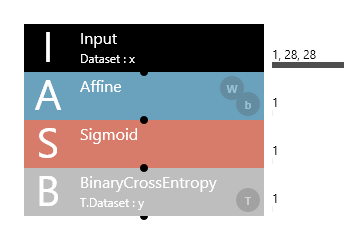
\includegraphics[width=\textwidth]{network_before_quant.png}
    \caption{Before}
    \label{subfig:before_quant_nnc}
  \end{subfigure}
  \quad % hfill
  \begin{subfigure}[b]{0.64\textwidth}
    \centering
    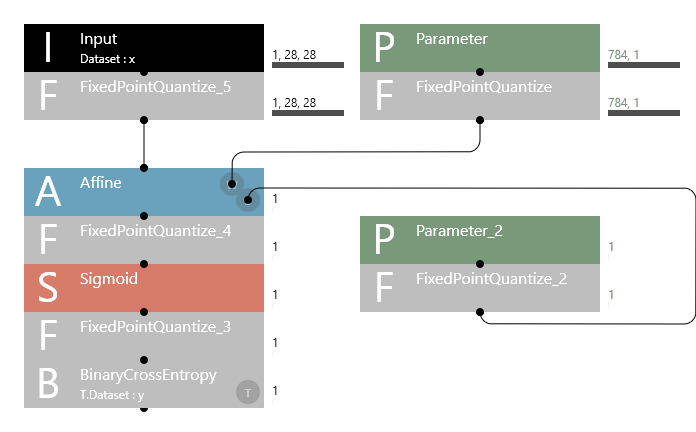
\includegraphics[width=\textwidth]{network_after_quant.png}
    \caption{After}
    \label{subfig:after_quant_nnc}
  \end{subfigure}

  \caption{Example of quantization in Neural Network Console}%
  \label{fig:quant_in_nnc}
\end{figure}

\Figref{fig:quant_in_nnc} shows the example of quantization in Neural Network Console. As the image shows, the FixedPointQuantize layer is inserted between other layers to quantize activations, and it is inserted in front of the parameter layer to quantize parameters. In this method, we were able to quantize all parameters and activations.

% \begin{equation} % \label{eq:quant}
The following equation is the equation we covered in section \ref{sec:implementation_operations}. In the case study, we quantized all parameters and activations to 8-bit integers, and we set the quantization step size ($\delta$) as the power of two.

\[
\textrm{quantized data in original scale} = \textrm{quantized data} \times \delta, \quad \delta = 2^{-n} \; \left( n = 1, 2, \ldots\right)
\]
% \end{equation}
`quantized data' is integer in the equation and $\delta$ stands for the size of 1 bit.
Since we are using $\delta$ as the power of two, we can calculate between the quantized data with low cost while implementing to FPGA. It is because we can use the shift operator for adjusting $\delta$. The detail with the operation with quantized numbers is discussed in section \ref{sec:implementation_operations}.

% However, if we use shift operations as division, it will discard the remainder. In the case of division, we add a number before shift operation to avoid this.


\subsection{Training and Accuracy} \label{sec:training_and_accuracy}
We use MNIST dataset \cite{mnist} to train and evaluate the networks. \Tabref{tab:number_mnist} shows the number of images used for training and evaluation. The accuracy measured in the evaluation are also listed in the same table.

  \begin{table}[tbp]
    \centering
    \caption{The number of images used and accuracy of the network}
    \label{tab:number_mnist}
    \begin{tabular}{l|rrrr}
      \hline\hline
      Network             & Training & Evaluation & Epoch & Accuracy \\
      \hline
      Logistic regression &  1,500   &    500     & 100   & 95.2 \% \\
      Binary CNN          &  1,500   &    500     & 100   & 98.0 \% \\
      LeNet               & 60,000   & 10,000     & 10    & 99.2 \% \\
      \hline
    \end{tabular}
  \end{table}



% \section{Implementation to FPGA}
\section{Implementation process flow}

\subsection{Preparing input data}
As we have discussed in section \ref{sec:training_and_accuracy}, we use the MNIST dataset to train and evaluate. Neural Network Console downloads and converts the MNIST dataset in PNG format to use it. We use the same PNG format of the MNIST dataset to make it easier to compare the inference results. Our main purpose is not on reading PNG images but implementing a network in FPGA. Therefore, we convert the PNG image to text for development convenience.

To prepare the image as a text, we read each pixel of an image. For the convenience of reading pixels of an image, we convert the image to BMP format. We can have the same image data because PNG and BMP are both lossless formats. We use a tool named ImageMagick \cite{imagemagick}. Following command was used.

\begin{quote}
  \begin{lstlisting}[language=bash, numbers=none, frame=l]
convert -compress none <input>.png <output>.bmp
  \end{lstlisting}
\end{quote}

The `\texttt{-compress none}' option defines not to compress the image. It is required because by default ImageMagick version 7.0.10.58 compress BMP image with a run-length encoding algorithm, making it harder to read pixels.

\begin{figure}[tbp]
  \centering
    \begin{tabular}{|p{2cm}|p{2cm}|}
    \hline
     \hfil Signature & \hfil\\
    \hline
    \multicolumn{2}{|c|}{File Size}\\
    \hline
     \hfil Reserved & \hfil Reserved\\
    \hline
    \multicolumn{2}{|c|}{File Offset to The Pixel Array}\\
    \hline
   \end{tabular}
  \caption{Bitmap File Header}
  \label{fig:bmp_header}
\end{figure}

Next, we built the program that reads each pixel of the BMP image to print it. Since the image data is not compressed, the program can open the image as binary and just read each pixel. \Figref{fig:bmp_header} shows the file header structure of BMP file. The width of the figure is 4 bytes. Therefore, the BMP format stores the offset of the pixel array at 0x0A. After reading the offset in the header, we are able to access its data.

\subsection{Preparing parameters}

After modifying the network in section \ref{sec:quantization}, and training in section \ref{sec:training_and_accuracy}, we implement it to FPGA. NNC stores the network in a binary file called `\texttt{results.nnp}'. To extract the parameter from this file, we used \texttt{nnabla\_cli} \cite{sony-nnabla}. \texttt{nnbla\_cli} is the command-line interface of Neural Network Libraries, which NNC is built on. We ran the following command to decode parameters.

\begin{quote}
  \begin{lstlisting}[language=bash, numbers=none, frame=l]
nnabla_cli decode_param -p results.nnp -o output_dir
  \end{lstlisting}
\end{quote}

This command will print out the parameters as files to `\texttt{output\_dir/}'. Data of each \texttt{Parameter} layer will be created under the directory. For example, if we decode parameters of \textbf{Figure~\ref{subfig:after_quant_nnc}}, `\texttt{Parameter.txt}' and `\texttt{Parameter\_2.txt}' will be created. \Figref{fig:parameter} is an example of decoded parameter text files. It includes the first nine lines of the parameter file. The first line indicates the matrix size of the parameter, and from the second line, the contents are recorded.

As shown in this figure, NNC stores the parameter as a float. Therefore, we quantized it to integer and stores it for use in the implementation. The parameter will be implemented as a C array in the hardware processes.

\begin{figure}[tbp]
  \centering
  \lstinputlisting[
  linerange={1-9},
  firstnumber=1,
  ]{"src/Parameter.txt"}
  \caption{Example of decoded parameter}
  \label{fig:parameter}
\end{figure}


\subsection{Designing functional units and the SDF file}

We design functional units and the SDF file as discussed in chapter \ref{sec:model_design}. After designing the functional units and SDF, we simulated the design.



% We designed a software process to send image data to FPGA, send start signals, receive results, and measure the time until receiving results. For the hardware unit, we designed it to receive the input image data and to return the inference value to the software.

% We design a System DeFinition (SDF) file for the declaration of the communication primitive between each unit. \Figref{fig:eg_sdf} is an example of the SDF file we designed for LeNet. As the figure shows, we used blocking communication primitive for communicating each hardware unit and memory primitives to commute the input image. After designing the functional units and SDF, we simulated the design.
% Due to space limitations, this figure contains only part of the file.

\subsection{Functional level simulation}
To test the design at a functional level, we simulate the design by synthesizing all units as software processes. It is useful for testing the output result of the design. If all units were synthesized as software, simulation time could be shortened since it does not go through a process such as high-level synthesis of hardware or emulating hardware using an RTL simulator.

% testing the design using co-simulation or real-machine demands more time.  However

We created a new SDF file that declares all functional units in software processes to run this simulation. We synthesize the design with the following command.

\begin{quote}
\begin{lstlisting}[language=bash, numbers=none, frame=l]
SysGen -sdfy <SDF file> -dobs -s zybo_z7_20 -bst vivado
\end{lstlisting}
\end{quote}

Each option of the command is discussed in section \ref{sec:command}. The RTOS is not specified in the command, but ITRON is used as a default for this board.

The command specifies to perform HLS. However, since there is no hardware process declared in the SDF file, HLS will not occur in this process. The command will create a new directory with the value declared as the system name (e.g. line 1 in \Figref{fig:eg_sdf}). For the functional level simulation, we use \emph{sp} as the system name. The directory `\texttt{sp/}' now has a result of synthesis. Next we change our working directory to `\texttt{\textit{sp}/fmp/}'. Then we simulate the design with the following command.

\begin{quote}
\begin{lstlisting}[language=bash, numbers=none, frame=l]
make runq
\end{lstlisting}
\end{quote}

This command compiles the software processes and runs QEMU to emulate RTOS with software processes. Next, we compare the received results with inference from NNC to determine whether the inference results were the same.

\subsection{Co-simulation}

% After testing the inference results in functional level simulation,
To debug the design, we run co-simulation. In the SDF file, the inference function must be partitioned as a hardware process in order to test the hardware behavior. To distinguish this design from the previous design in functional level simulation, we use \emph{sp\_hw} as the system's name, which indicates that the system has hardware processes.

Next, we synthesize the design with the same command discussed in functional level simulation. Unlike in the functional level simulation, we have declared the hardware processes. Therefore this command runs the HLS tool. We use Vivado for high-level synthesis.

\begin{quote}
\begin{lstlisting}[language=bash, numbers=none, frame=l]
SysGen -sdfy <SDF file> -dobs -s zybo_z7_20 -bst vivado
\end{lstlisting}
\end{quote}

 After changing the working directory to `\texttt{sp\_hw/fmp/}', we executed the following commands.

\begin{quote}
\begin{lstlisting}[language=bash, numbers=none, frame=l]
make runsim &
make runq
\end{lstlisting}
\end{quote}

The first command runs Questa Sim. Questa Sim compiles HDL files and simulates the hardware, and the second command compiles the software processes and runs QEMU to emulate the software processes. Next, we check the signal wave to debug the design. We run the following commands at Questa Sim's transcript.

\begin{quote}
\begin{lstlisting}[language=bash, numbers=none, frame=l]
add wave -position end sim:/sp_hw/*
\end{lstlisting}
\end{quote}

The wave window will now print the signal wave on its window. Then, we ran the following commands at Questa Sim's transcript to start the RTL simulation.

\begin{quote}
\begin{lstlisting}[language=bash, numbers=none, frame=l]
run -all
\end{lstlisting}
\end{quote}

Finally, after sending a start signal at QEMU, we observe the result of co-simulation.

\subsection{Implementation on the real-machine}

After co-simulation, we implement the design on the real-machine to test inference and performance. Like other processes discussed above, we synthesize the entire design and high-level synthesize the hardware with the following command.

\begin{quote}
\begin{lstlisting}[language=bash, numbers=none, frame=l]
SysGen -sdfy <SDF file> -dobs -s zybo_z7_20 -bst vivado
\end{lstlisting}
\end{quote}

Next, we run logic synthesis. SystemBuilder provides Vivado's batch script for logic synthesis. To use this, copy the files in `\texttt{Zynq/ZYBO\_Z7\_20/}' of the SystemBuilder installation path to `\texttt{sp\_hw/zynq/}' and run \texttt{run.sh}.

After logic synthesis, we connect the FPGA board to the computer and run the following command as the root account. This command implements the bitstream on the real-machine.

\begin{quote}
  \begin{lstlisting}[language=bash, numbers=none, frame=l]
make runf
  \end{lstlisting}
\end{quote}

Next, we communicate with the serial port to obtain the results. To communicate with the serial port on Linux, we did the following:

Suppose FPGA board's serial port is connected to `\texttt{/dev/ttyUSB1}'. We run the following command as the root account to display `\texttt{/dev/ttyUSB1}'.

\begin{quote}
  \begin{lstlisting}[language=bash, numbers=none, frame=l]
screen /dev/ttyUSB1 115200
  \end{lstlisting}
\end{quote}

This command connects `\texttt{/dev/ttyUSB1}' with baud rate at 115200.
Then we are able to communicate with the board via GNU Screen.


\section{Design decision of each case study} \label{sec:design_case_study}
\subsection{Logistic regression} \label{sec:logistic_regerssion}

\begin{figure}[tb]
  \center
  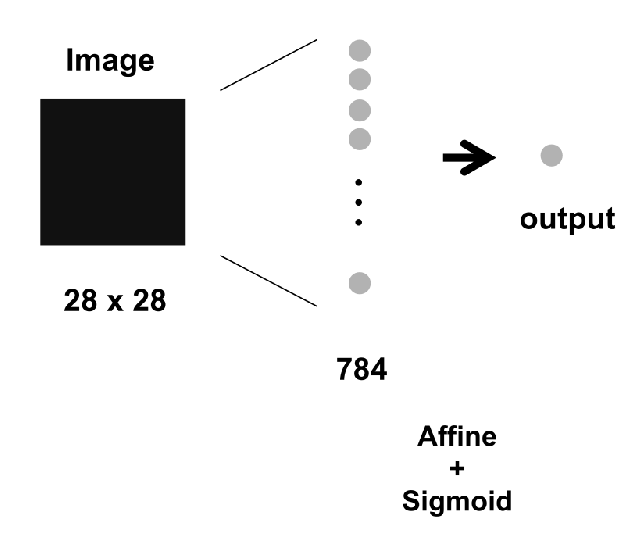
\includegraphics[width=0.41\textwidth]{affine.eps}
  \caption{Logistic regression.}
  \label{fig:affine}
\end{figure}

Logistic regression is a simple network that is formed with two layers. This network can be referred to from \Figref{fig:affine}. For hardware design, we use \textbf{Design 1} discussed in section \ref{sec:overall_design}. This hardware design is to use a single hardware process with multiple functions inside. Logistic regression is the first case study with the top priority of implementing it in an FPGA. Single hardware process design is simple comparing with multiple hardware processes design. Thus it is relatively effortless to implement the model.

To implement the activation function, we use the Taylor series of activation function that can be referenced in \cite{ccetin2015application}. However, we could not obtain the correct result by following the equation in \cite{ccetin2015application}. We expect this is because the calculations have occurred with the low precision of 8-bit integers. We made exception handling for the input that did not match the correct result to solve this problem.


\subsubsection{Pipelining the loop}

\begin{figure}[tbp]
  \centering
  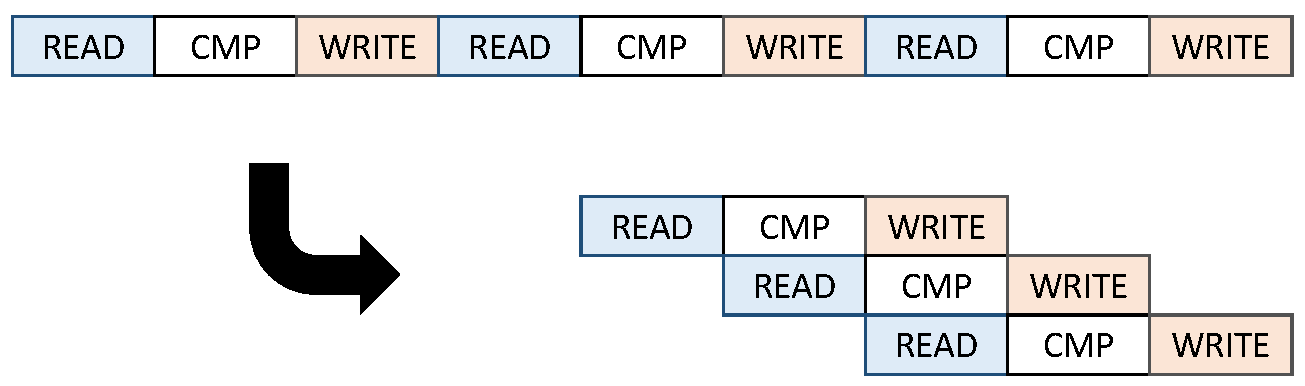
\includegraphics[width=0.89\textwidth]{pipelining_loop.pdf}
  \caption{Image of pipelining the loop}%
  \label{fig:pipelining_loop}
\end{figure}

We use a loop statement to implement the matrix multiplication in an affine layer. We have tested pipelining this loop statement using HLS. \Figref{fig:pipelining_loop} depicts the concurrent execution by pipelining operations, which will shorten the computation time. Its effectiveness will be discussed in the results (section \ref{sec:results}).
% is an image of pipelining showing that implementing the operations in a concurrent manner.
% Using the HLS tool, pipelining such as the figure has applied. This will shorten the computation time. Its effectiveness will be discussed in the results (section \ref{sec:results}).

%%%%%
% After implementation, we tested the performance using pipelining and unrolling which HLS tools provided. The results refer as \ref{tab:result}.
%%%%%

\subsection{Binary CNN}\label{sec:binarycnn}

\begin{figure*}[tbp]
  \center
  \includegraphics[width=0.99\textwidth]{network_fixed.eps}
  \caption{Binary CNN}
  \label{fig:binary_cnn_network}
\end{figure*}

After successful implementation of logistic regression in section \ref{sec:logistic_regerssion}, we implement another network.
We search for the DNN Model, which includes the convolution layer. It is because we think that the convolution layer has room for further optimization with a loop statement. This room could help to test the HLS tool's optimization as future work. We use binary CNN from example networks provided by NNC \cite{webpage:nnc_project}. This network can be referred from \Figref{fig:binary_cnn_network}.

For hardware design, we use \textbf{Design 2} discussed in section \ref{sec:overall_design}. This hardware design is to use a multiple hardware process that plays each layer's role. As discussed in section \ref{sec:overall_design}, we build six hardware processes for binary CNN, corresponding to two convolution layers, two max-pooling layers, and two affine layers. Other layers are designed to be built-in to the previous layer. The reason for this design is that it will be able to test the pipelining at the layer level, which will be discussed later.

We use a lookup table for the activation layer such as Tanh and Sigmoid. As discussed in section \ref{sec:logistic_regerssion}, calculating the activation function with the low precision of 8-bit integers is challenging to achieve the correct result.

\subsubsection{Pipelining the process} \label{sec:bin_pipe}

\begin{figure}[tbp]
  \centering
  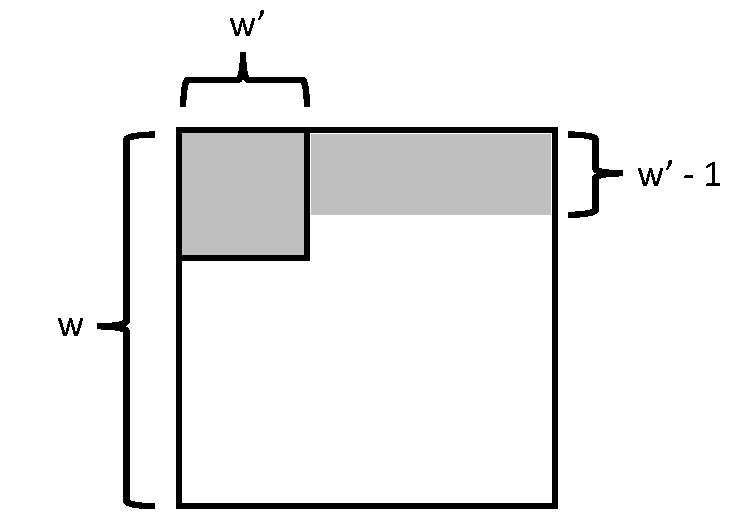
\includegraphics[width=0.4\linewidth]{pipelining_layer_buffer_size.pdf}
  \caption{Image of buffer size}%
  \label{fig:buffer_size}
\end{figure}

In the implementation of binary CNN, we use six hardware processes. Separating the hardware processes makes it possible to pipeline at the process level. We design each process to accumulate input data in a buffer until one operation is possible. When there is enough data in the buffer, it executes the operation and export the result. \Figref{fig:buffer_size} depicts this process. Suppose the outer square presents the input matrix and the inner square presents the kernel matrix.
The colored part of the figure should be accumulated in the buffer to calculate one element of the output matrix. The size of the colored part is as follows:
\[w * (w' -1) + w'\]
This will be the size of the buffer. After calculating one output element, the buffer should be shifted to store the next input element. In a case like \Figref{fig:buffer_size}, the buffer will be shifted by $w'$. After shifting, the buffer will receive a new input element. Likewise, if the buffer is full, the calculation of one output element will occur.

The method described above is slightly different from the actual implementation. The max-pooling layer is implemented in the same way as above, but the convolution layer is different. In the case of the convolution layer of binary CNN, the input matrix is three dimensions, and the kernel is also three dimensions. The concept of accumulating the buffer is the same, though there is no shifting to discard unnecessary elements. This is because unnecessary elements are not arranged in the first few elements as in two dimensions, which disallows discarding.

Using this method, we are able to pipeline the processes. We compare the pipelined and non-pipelined results.



\subsection{LeNet}
\begin{figure}[tbp]
  \centering
  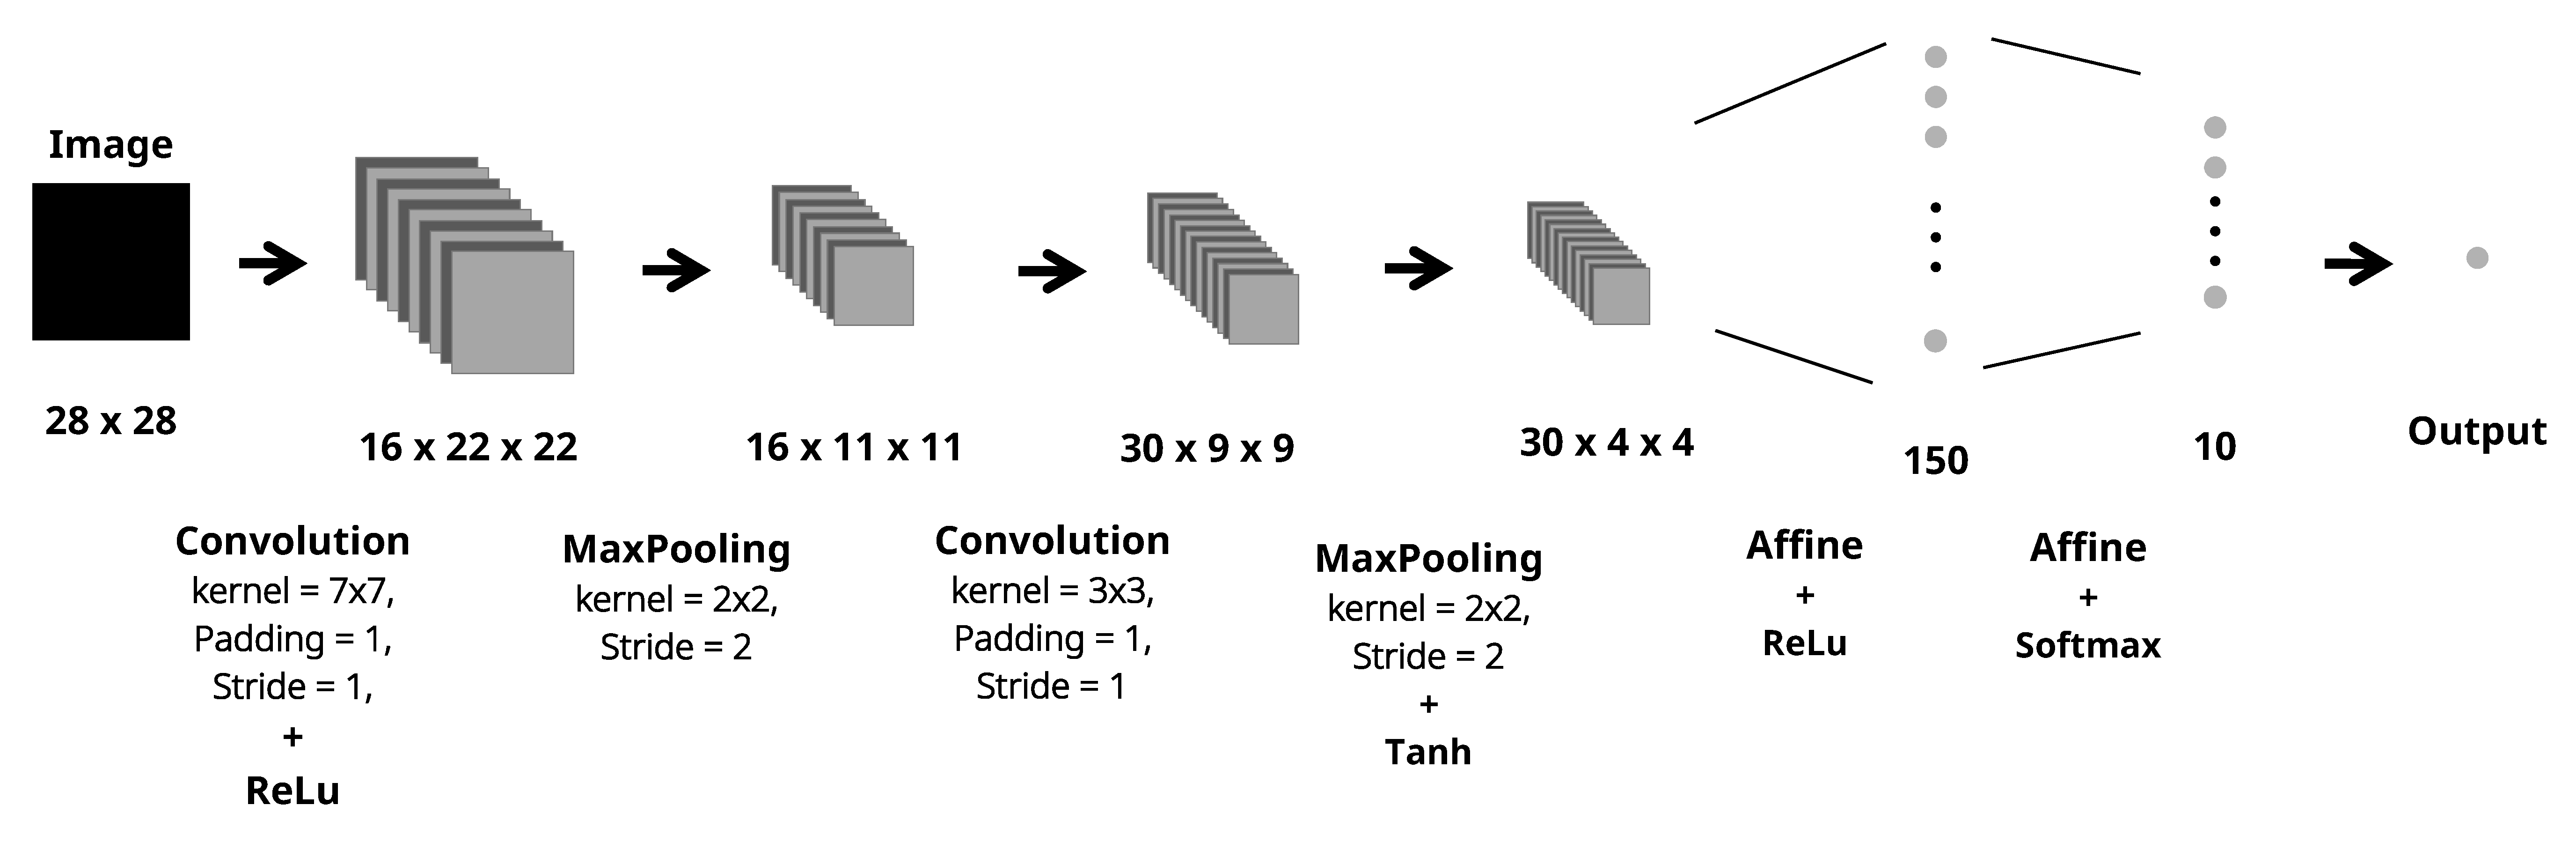
\includegraphics[width=0.99\linewidth]{LeNet.pdf}
  \caption{LeNet}%
  \label{fig:lenet}
\end{figure}
For the final case study, we implement the LeNet. Unlike the other two, LeNet classifies ten kinds of input data. This network can be referred to from \Figref{fig:lenet}.

As with the design of binary CNN, we use six hardware processes to pipeline the process. We use a lookup table for the Tanh activation function. In the case of ReLu, we followed the definition of the function: if the input value is below 0, the output is 0.

\section{Results} \label{sec:results}
\subsection{Logistic regression and binary CNN}

\begin{table}[tbp]
  \caption{A result of case study including loading time of input image.}
  \label{tab:result}
  \begin{adjustwidth}{-2in}{-2in}
    \centering
    \begin{tabular}{rl|rrrr}
      \hline\hline
      Network              & Optimization     &      Latency & Throughput & BRAM Usage & LUT as Logic Util Rate\\
      \hline
      \multirow{2}{*}{
      Logistic regression} & -                &   347 $\mu$s & 2884 fps & 162 kB & 16.06 \% \\
                           & pipeline (loop) &   330 $\mu$s & 3031 fps & 162 kB & 16.61 \% \\
      \multirow{2}{*}{
      Binary CNN}          & -                & 18772 $\mu$s & 53.3 fps & 200 kB & 18.19 \% \\
                           & pipeline (process) & 18092 $\mu$s & 55.3 fps & 180 kB & 18.65 \% \\
      \hline
      \multicolumn{6}{l}{Target: ZYBO@100MHz}\\
      \multicolumn{6}{l}{Latency for Logistic regression\,: {\tt average execution time of 100-discussion}}\\
      \multicolumn{6}{l}{Latency for Binary CNN\,: {\tt average execution time of 10-discussion}}\\
    \end{tabular}
  \end{adjustwidth}
              % & & unroll   &   326 &  3066 & 160 \\
\end{table}

\begin{table}[tbp]
\caption{A result of case study without loading time of input image.}
\label{tab:result2}
  \begin{adjustwidth}{-2in}{-2in}
    \centering
    \begin{tabular}{rl|rrrr}
      \hline\hline
                   Network & Optimization & Latency & Throughput & BRAM Usage & LUT as Logic Util Rate \\
      \hline
      \multirow{2}{*}{
      Logistic regression} & -                &  61.5 $\mu$s & 16260 fps & 162 kB & 16.60 \% \\
                           & pipeline (loop) &  45.5 $\mu$s & 21978 fps & 162 kB & 16.61 \% \\
      \multirow{2}{*}{
      Binary CNN}          & -                & 18489 $\mu$s &  54.1 fps & 200 kB & 15.23 \% \\
                           & pipeline (process) & 17809 $\mu$s &  56.2 fps & 180 kB & 15.68 \% \\
      \hline
      \multicolumn{6}{l}{Target: ZYBO@100MHz}\\
      \multicolumn{6}{l}{Latency\,: {\tt execution time for 1-discussion}}\\
    \end{tabular}
  \end{adjustwidth}
                                     % & & unroll   &   326 &  3066 & 160 \\
\end{table}


For logistic regression and Binary CNN, we have confirmed that our implementation shows the same inference as the original. Next, we measure the performance of our implementation. We measure two kinds of data. One is the total latency from data transmission to output of the FPGA. This data is listed in \Tabref{tab:result}. We calculate the average of 100 inferences for logistic regression, and for Binary CNN, we use the average of 5 inferences. The other measured performance is latency without input data transmission latency, which is the network's pure computation latency. This data is listed in \Tabref{tab:result2}

The optimization column in these tables is information for comparing the applied optimization method. `pipeline (process)' means that it pipelined at the process level, and `pipeline (loop)' means that it pipelined one loop statement. This optimization method is discussed in section \ref{sec:design_case_study}.

We have tested the optimization technique in the logistic regression's implementation using the HLS tool described in section \ref{sec:hwsynthesis}. We have pipelined the loop statement in the affine layer. As a result, the throughput improved from 2884 fps to 3031 fps, resulting in a five percent performance improvement (\Tabref{tab:result}).  However, focusing on the computation time itself, throughput improved from 16260 fps to 21978 fps, resulting in a 35 percent performance improvement (\Tabref{tab:result2}).

In the implementation of Binary CNN, we experiment with pipelining in processes. As a result, throughput increased from 53.3 fps to 55.3 fps, resulting in a 3.8 percent performance improvement (\Tabref{tab:result}). Performance improvement focusing on the computation time itself was increased from 54.1 fps to 56.2 fps, resulting in a 3.9 percent performance improvement (\Tabref{tab:result2}).

\subsection{LeNet}
In the implementation of LeNet, the inference results did not match with the NNC. When we check the inference result of 10000 images, six were different from NNC.

\section{Discussion}
\subsection{The communication time}
% Comparing \Tabref{tab:result} and \Tabref{tab:result2}, it shows a laten a difference in latency of approximately 284 $\mu$s.
% This latency is the time required for the FPGA to read the image from memory.
When comparing the latencies in \Tabref{tab:result} with the latencies in \Tabref{tab:result2}, there is a consistently constant difference of about 284 $\mu$s. We believe that this consistently constant difference of latency is the time require for image data transmission to the FPGA.

The latency of binary CNN, including data transmission, is 18489 $\mu$s (without pipelining). 284 $\mu$s is about 1.0 percent of the entire latency for binary CNN. However, the entire latency of logistic regression is 374 $\mu$s (without pipelining), which leads to 284 $\mu$s to be about 82 percent of the entire latency for logistic regression. Transferring of input data is being a huge bottleneck for logistic regression. Testing other communication primitives such as prefetch BC will be worthy as future work.

\subsection{Activation function}
% Implementing a sigmoid layer or a Tanh layer from the definition might require the implementation of the exponential function. However, implementing an exponential calculation of quantized numbers was a difficult task for us.  Consequently,
We built the sigmoid function using the Taylor series in section \ref{sec:logistic_regerssion}. We suspected the loss using the Taylor series would be negligible. We thought the loss in quantizing the results would be much bigger to be able to hide the loss in the Taylor series. We used multiple Taylor series for multiple domains. We found out that the output does not monotonically increase at the boundary of each domain. We expect this is due to the low precision calculations of 8-bit integers.


To solve this problem, we took a different approach in section \ref{sec:binarycnn}. We prepared 256 ($ = 2^8$) size output an array that corresponds to 256 cases of input. We made a lookup table.

Apart from the difficulty of making, but in terms of performance and circuit size, we believe that comparing the lookup table and implementing it as a function is worthy of discussion.

\subsection{Pipelining}
\subsubsection{Observed waveform of binary CNN}
In binary CNN, we have tested the pipelining at the process level. We observed the waveform to debug its behavior.

\Figref{fig:waveform_pipeline} shows the signal between hardware processes conv1, mpool1, and conv2. These processes represent convolution, max-pooling, and convolution layer. The signal in the figure represents data transmission between processes. The signal marked as two in \Figref{fig:waveform_pipeline} represents the data transmission from mpool1 to conv2. As \Figref{fig:waveform_pipeline} shows, there is a gap between data transmission between mpool1 and conv2. This gap's latency represents the latency of accumulating the buffer of the mpool1 process. This figure shows the mpool1 process begins to calculate and print output element to next process after accumulating input element.

\Figref{fig:waveform_n_pipeline} is a waveform of binary CNN which is not pipelined. In \Figref{fig:waveform_n_pipeline}, mpool1 prints output element after receiving all input elements from conv1. This is clearly different behavior from \Figref{fig:waveform_pipeline}.

However, there is a limitation on our process level pipelined model. \Figref{fig:waveform_pipeline_overview} shows the same model as \Figref{fig:waveform_pipeline} but with larger scale. The gap marked as one is a latency before the conv2 process begins to print the result. \Figref{fig:waveform_pipeline_overview} shows conv2 begins to print result after receiving most of the mpool1's output. The convolution process of our DNN model receives three dimensions of the input matrix. Moreover, the convolution process requires matrix multiplication of a kernel matrix with the same depth as the input matrix. This leads requiring of accumulating most of the elements in the pipelining design.


\begin{figure}[tbp]
  \centering
  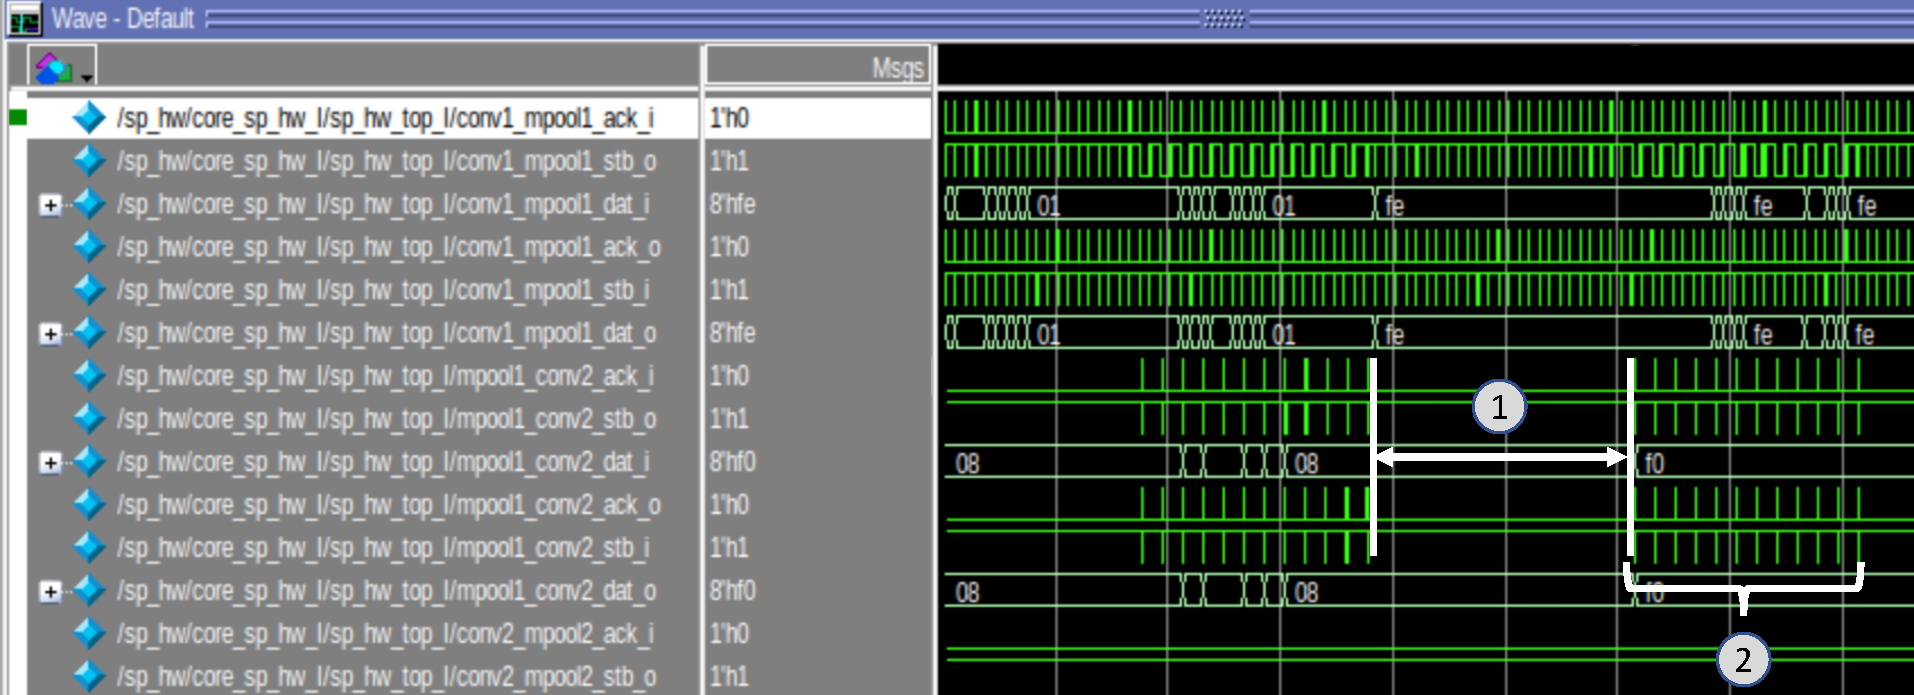
\includegraphics[width=0.96\linewidth]{per_pixel_detail.pdf}
    \begin{tabular}{l}
      1: Latency of accumulating the buffer at mpool1 process. \\
      2: Data transmission from mpool1 to conv2.
    \end{tabular}
  \caption{The waveform of the model pipelined at the process level}
  \label{fig:waveform_pipeline}
\end{figure}

\begin{figure}[tbp]
  \centering
  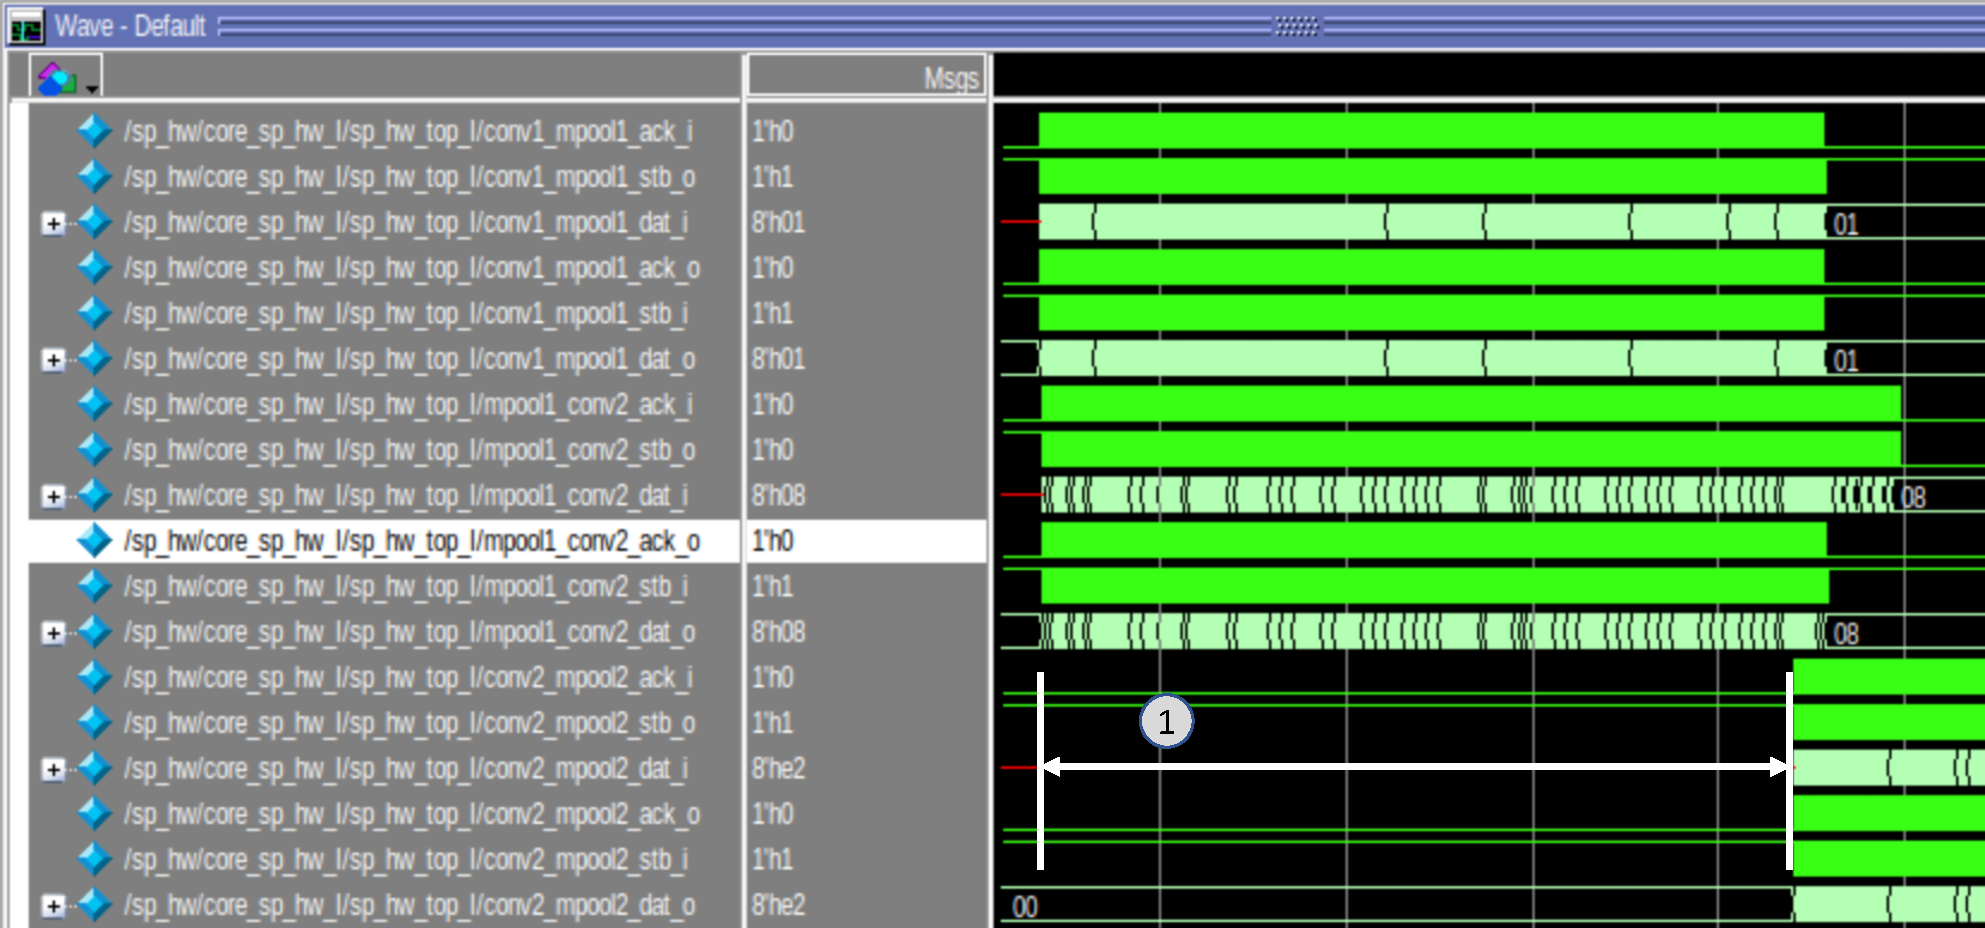
\includegraphics[width=0.99\linewidth]{per_pixel_big.pdf}
    \begin{tabular}{l}
      1: Latency of accumulating the buffer at conv2 process. \\
    \end{tabular}
  \caption{The overview waveform of the model pipelined at the process level}
  \label{fig:waveform_pipeline_overview}
\end{figure}

\begin{figure}[tbp]
  \centering
  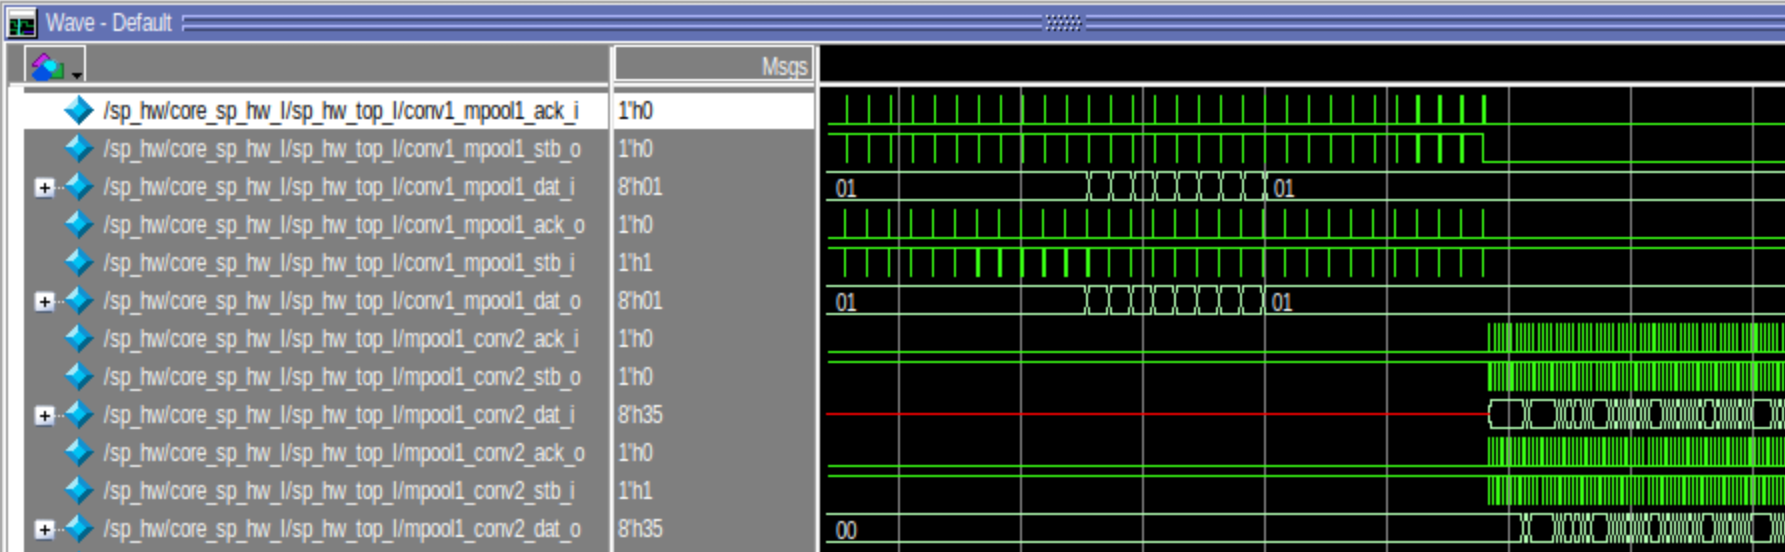
\includegraphics[width=0.99\linewidth]{per_image_detail.png}
  \caption{The waveform of the model that did not pipeline the process}
  \label{fig:waveform_n_pipeline}
\end{figure}

\subsubsection{Efficiency}

In order to discuss the efficiency of the pipelining, we will discuss the performance gains and the increased LUT usage from pipelining. We will discuss the performance gain with the result without data transmission of an input image, represented in \Tabref{tab:result2} and discussed in section \ref{sec:results}.
% In the implementation of logistic regression, by pipelining one loop in the layer, there was about 35 percent improvement in computation speed.

\subparagraph{Logistic regression}
% In the implementation of logistic regression,
We observe about 35 percent improvement of computation speed by pipelining on loop in the process. At the same time, logic LUT usage rate increased from 16.60 \% to 16.61 \% (\Tabref{tab:result2}). The increase is about 0.1 percent. We believe that it showed high-efficiency use of logic LUT when considering the performance improvement. The amount of BRAM usage is the same as 160 kB.
% The increase in the logic LUT usage rate was 0.1 percent (\Tabref{tab:result2}).

\subparagraph{Binary CNN}
% In the implementation of binary CNN,
We observe about 3.9 percent performance improvement by pipelining at the process level. At the same time, logic LUT usage rate is increased from 15.23 \% to 15.68 \% (\Tabref{tab:result2}). The increase is about 0.45 percent. It is relatively inefficient compared to the above case, considering the degree of performance improvement.

However, BRAM usage has decreased from 200 kB to 180 kB, which can be said it is an advantage of the optimization. We suspect the BRAM has decreased because the buffer accumulating the previous layer results has decreased in each process.

\subsection{Problems of LeNet}

\begin{figure}[tbp]
  \centering
  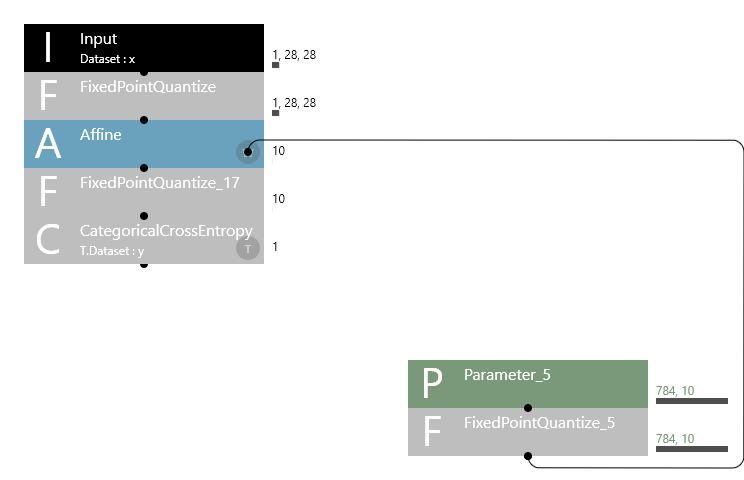
\includegraphics[width=0.7\linewidth]{network_affine_only.png}
  \caption{Affine layer-only network}%
  \label{fig:network_affine}
\end{figure}
In the results, we found out the inference results of LeNet were different from NNC in few cases. To find out the cause, we did the following:

To find out the result of one matrix multiplication, we design a network only with one affine layer and quantization layers, as \Figref{fig:network_affine}. If we disable the affine layer's bias, the output will be the result of multiplying the input matrix and parameter matrix. This result can make us understand the matrix multiplication behavior in NNC. Matrix multiplication is also used in the convolution layer. Therefore, observing a single affine layer can help us understand the overall operation of NNC.
% This network can be referred to from \Figref{fig:network_affine}.


Next, we implement this network in the same method as the case study. When comparing the result (matrix), about half of the matrix elements showed different values. The error is at most 1; hence it is not a big error. However, we believe the accumulation of errors during the operation results in difference in the output for some cases.

The reason for the error was not known.
